%\documentclass[11pt]{article}  % for e-submission to ApJ
\documentclass[11pt]{NSF}  % for e-submission to ApJ


\usepackage{graphicx, natbib, color, bm, amsmath, epsfig}
\usepackage{wrapfig}

%paper commands, for when not using aastex
\newcommand\physrep{Phys.~Rep.}
\newcommand\fcp{Fund.~Cosmic~Phys.}
\newcommand{\pre}{Phys Rev E}
\newcommand{\apj}{ApJ}
\newcommand{\apjs}{ApJS}
\newcommand{\aj}{AJ}
\newcommand{\aap}{A\&A}
\newcommand{\mnras}{MNRAS}
\newcommand{\araa}{ARA\&A}
\newcommand{\procspie}{Proc.SPIE}
\newcommand{\pasj}{PASJ}
\newcommand{\iaucirc}{IAU Circ.}
\newcommand{\aplett}{AP Letters}
\newcommand{\aaps}{AAPS}
\newcommand{\aapr}{AAPR}
\newcommand{\nat}{Nature}
\newcommand{\apjsupp}{ApJS}
\newcommand{\pasp}{PASP}
\newcommand{\apjl}{ApJL}
\newcommand\prl{Phys.~Rev.~Lett.}
\newcommand\apss{Ap\&SS}




%%%% PUT NEW COMMANDS AND DEFINITIONS HERE %%%%
\usepackage{graphicx, natbib, color, bm, amsmath, epsfig}

%
% Hijacked and hacked from aastex.cls
%
%\def\newblock{\hskip .11em\@plus.33em\@minus.07em}%

%\newcommand\plotone[1]{%
% \typeout{Plotone included the file #1}
% \centering
% \leavevmode
% \includegraphics[width={\eps@scaling\columnwidth}]{#1}%
%}
%\newcommand\plotone[1]{
% \includegraphics[width=3.0in]{#1}%
%}
%\let\tableline=\hline
%enzo commands
\newcommand\jcompphys{J.~Comput.~Phys}
\newcommand\physfluidsa{Phys.~Fluids~A}
\newcommand\physfluids{Phys.~Fluids}
\newcommand\physlettA{Phys.~Lett.~A}
\newcommand\jfm{J.~Fluid~Mech.}
\newcommand\ccm{Comput.~Phys.~Commun.}
\newcommand\jphysique{J.~Physique~I}
\newcommand\revmodphys{Rev.~Mod.~Phys.~}

%\newcommand\aap{\ref@jnl{A\&A}}% 
%\newcommand\prb{\ref@jnl{Phys.~Rev.~B}}% 
          % Physical Review B: Solid State 


\newcommand{\ratio}{\mathcal{R}}
\newcommand{\yt}{{\tt yt}}
\newcommand{\Lmax}{\ell_{\rm max}}
\newcommand{\enzo}{{\small Enzo}}
\newcommand{\menzo}{{EnzoMHD}}
\newcommand{\Menzo}{{EnzoMHD}}
\newcommand{\zeus}{{\small ZEUS}}
\newcommand{\Lbox}{L_{\rm box}}
\newcommand{\Nroot}{N_{\rm root}}
\newcommand{\K}{\,\rm K}
\newcommand{\dave}{DaveThena}
\newcommand{\grid}{{\tt grid}}

%\newcommand{\lct}[3]{\ensuremath{\epsilon_{#1,#2,#3}}}
\newcommand{\lct}[1]{\ensuremath{\epsilon_{#1}}}
%grid location commands.
\newcommand{\iph}{i + \frac{1}{2}}
\newcommand{\imh}{i - \frac{1}{2}}
\newcommand{\jph}{j + \frac{1}{2}}
\newcommand{\jmh}{j - \frac{1}{2}}
\newcommand{\kph}{k + \frac{1}{2}}
\newcommand{\kmh}{k - \frac{1}{2}}

\newcommand{\ipmh}{i \pm \frac{1}{2}}
\newcommand{\half}{\frac{1}{2}}
\newcommand{\quart}{\frac{1}{4}}
\newcommand{\tquart}{\frac{3}{4}}

%physics commands
\newcommand{\avir}{\ensuremath{\alpha_{\rm{vir}}}}
\newcommand{\mach}{\ensuremath{\mathcal{M}}}
\newcommand{\hmag}{\ensuremath{H_{\rm{M}}}}
\newcommand{\alfmach}{\ensuremath{\mathcal{M_{\rm{A}}}}}
%\newcommand{\msun}{\ensuremath{\rm{M}_\odot}}
\newcommand{\msun}{\ensuremath{M_\odot}}
\newcommand{\lsun}{\ensuremath{L_\odot}}
\newcommand{\rsun}{\ensuremath{R_\odot}}

\def\mch{\ensuremath{M_{\rm{Ch}}}}
\def\AD{{\rm{AD}}}

%math commands
\def\rms{\ensuremath{\rm{rms}}}
\newcommand{\pts}[1]{\emph{(#1 pts)}}
\newcommand{\dbd}[2]{\frac{ \partial #1 }{ \partial #2} }
\newcommand{\ddbd}[2]{\frac{ d #1 }{ d #2} }
\newcommand{\dDbD}[2]{\frac{ \mathrm{D} #1 }{ \mathrm{D} #2} }
\newcommand{\curl}{\nabla \times}
\newcommand{\divb}{\ensuremath{\nabla \cdot {\bvec}}}
\newcommand{\divv}{\ensuremath{\nabla \cdot {\vvec}}}
\newcommand{\divbo}{$\nabla \cdot {\bf B} = 0$}
\newcommand{\intd}[1]{\int_#1^{#1 + \Delta #1} }
\newcommand{\dt}{\Delta t}
\newcommand{\dx}{\Delta x}
\newcommand{\dy}{\Delta y}
\newcommand{\dz}{\Delta z}
\newcommand{\p}[1]{#1^\prime }
\newcommand{\pp}[1]{#1^{\prime \prime} }
\newcommand{\tff}{\ensuremath{t_{\rm{ff}}}}
\newcommand{\kkmin}{\ensuremath{k/k_{\rm{min}}}}
\newcommand{\kmax}{\ensuremath{k_{\rm{max}}}}

%dcc color commands
\definecolor{orange}{rgb}{1.        ,  0.54,  0}
\newcommand{\orange}[1]{\textcolor{orange}{#1}}

\newcommand{\gtt}[1]{\textcolor{green}{{\tt#1}}}
\newcommand{\red}[1]{\textcolor{red}{#1}}
\newcommand{\yellow}[1]{\textcolor{yellow}{#1}}
\newcommand{\blue}[1]{\textcolor{blue}{#1}}
\definecolor{meta}{rgb}{0.371,0.617,0.625} %cadet blue for
                                           %non-production worthy
                                           % discussion of the work
\newcommand{\meta}[1]{\textcolor{meta}{#1}}
\newcommand{\green}[1]{\textcolor{green}{#1}}
\newcommand{\aake}[1]{\textcolor{blue}{#1}}
\newcommand{\bld}[1]{\mathbf{#1}}

\def\here{\red{notes later}}
%\newcommand{\hilite}[1]{\textcolor{red}{#1}}
%\newcommand{\hilite}[1]{#1}

%\newcommand{\bold}[1]{{\bf #1}}
%the comment maker, dc: the first one will show all comments in green, 
%the second hides them all.
%\newcommand{\dc}[1]{\textcolor{green}{#1}}
\newcommand{\dc}[1]{}
%\newcommand{\dc}[1]{#1}
%\def\bvec{\ensuremath{\vec{B}}}
%\def\vvec{\ensuremath{\vec{v}}}
\def\Bvec{\ensuremath{{\bf B}}}
\def\Jvec{\ensuremath{{\bf J}}}
\def\Avec{\ensuremath{{\bf A}}}
\def\bvec{\ensuremath{{\bf b}}}
\def\vvec{\ensuremath{{\bf v}}}
\def\uvec{\ensuremath{{\bf u}}}
\def\rvec{\ensuremath{{\bf r}}}
\def\xvec{\ensuremath{{\bf x}}}
\def\kvec{\ensuremath{{\bf k}}}
\def\Omegavec{\ensuremath{{\bf \Omega}}}
\def\omegavec{\ensuremath{{\bf \omega}}}
%\newcommand{\BlockOut}[1]{}
\newcommand{\BlockOut}[1]{#1}
\newcommand{\imp}{\ensuremath{\implies}}
\newcommand{\question}[1]{\textcolor{red}{#1}}
\definecolor{pink}{rgb}{1.        ,  0.75294118,  0.79607843}
\definecolor{maroon}{rgb}{0.69019608,  0.18823529,  0.37647059}
\newcommand{\ToRead}[1]{\textcolor{maroon}{#1}}
\newcommand{\ToReadUrgent}[1]{\textcolor{red}{#1}}
\newcommand{\HaveRead}[1]{\textcolor{black}{#1}}
\newcommand{\Old}[1]{\textcolor{blue}{#1}}
\newcommand{\Scanned}[1]{\textcolor{meta}{#1}}
\newcommand{\dccnote}[1]{}
%\newcommand{\dccnote}[1]{\textcolor{red}{#1}}
\def\nn{\nonumber}

\newcommand{\get}[1]{\textcolor{red}{#1}}
\definecolor{gray}{rgb}{0.5,0.5,0.5}
\newcommand{\gray}[1]{\textcolor{gray}{#1}}
\newcommand{\clean}[1]{\textcolor{gray}{#1}}
\newcommand{\ToDo}[1]{\textcolor{red}{#1}}
\def\etal{{\sl et al.}}

%chemistry commands
\newcommand{\Htwo}{\ensuremath{\rm{H}_2}}
\newcommand{\twelveco}{\ensuremath{^{12}\rm{CO}}}
\newcommand{\thirteenco}{\ensuremath{^{13}\rm{CO}}}

\newcommand{\mhdlabel}{{_{MHD}}}
\newcommand{\gravlabel}{{_{Grav}}}
\newcommand{\fclabel}{{_{fc}}}
\newcommand{\explabel}{{_{exp}}}
\newcommand{\sci}[1]{\ensuremath{\times {10^{#1}}}}
\newcommand{\percc}{\ensuremath{\rm{cm}^{-3}}}
\newcommand{\gcc}{\ensuremath{\rm{g}\ \rm{cm}^{-3}}}
\newcommand{\kms}{\ensuremath{\rm{km}\ \rm{s}^{-1}}}
\newcommand{\cms}{\ensuremath{\rm{cm}\ \rm{s}^{-1}}}
\newcommand{\cmperg}{\ensuremath{\rm{cm}^{2}\ \rm{g}^{-1} }}
\newcommand{\cmcmpers}{\ensuremath{\rm{cm}^2\ \rm{s}^{-1} }}
\def\muG{\ensuremath{\mu\rm{G}}}
\def\micron{\ensuremath{\mu\rm{m}}}
\def\alf{Alfv\' en}
\def\Alfvenic{Alfv\' enic}
\def\sa{super-Alfv\' enic}
\def\Sa{Super-Alfv\' enic}
\def\suba{sub-Alfv\' enic}
\def\Suba{Sub-Alfv\' enic}
\def\transa{trans-Alfv\' enic}
\def\Transa{Trans-Alfv\' enic}
\def\cs{\ensuremath{c_{\rm{s}}}}
\def\va{\ensuremath{v_{\rm{A}}}}
\def\sfrff{\ensuremath{{\rm SFR_{ff}}}}
%\def\velocity{\ensuremath{\vec{v}}}
%\def\magnetic{\ensuremath{\vec{B}}}
\def\velocity{\ensuremath{{\bf v}}}
\def\magnetic{\ensuremath{{\bf B}}}
\newcommand{\Fourier}[1]{\ensuremath{\tilde{#1}}}
\def\hfw{0.49}
\def\hw{0.49}
\def\fw{0.9}

\def\ssp{\def\baselinestretch{1.0}\large\normalsize}

\def\rhoc{\ensuremath{\rho_{\rm{c}}}}
\def\erf{\ensuremath{\rm{erf}}}


\def\SUtotal{2.9\sci{5}       }%cut from table1.
\def\tfinal{T_{\rm{final}}}
\def\suzu{\ensuremath{\rm{SU}_{\rm{zu}}}}
\def\nzones{N_{\rm{z},\ell}}
\newcommand{\Lund}{\ensuremath{\mathrm{S}}}
%\newcommand{\SUestimate}[1]{\textcolor{red}{#1}}
\newcommand{\SUestimate}[1]{#1}
\def\SUtotal{1.6\sci{5}       }                                                       
%\def\SUturb{1.8\sci{4}}
%\def\SUcore{1.2\sci{4}}
%\def\SUcmb{2.6\sci{4}}
%\def\SUgal{2.2\sci{3}}
%\def\DiskTurb{5.6\sci{3} Gb}
%\def\DiskCore{1.6\sci{5} Gb}
%\def\Diskcmb{1.7\sci{4} Gb}
%\def\Diskgal{1.1\sci{4} Gb}
%\def\StoreTotal{1.9\sci{5} Gb}
\def\nameTurbulence{\emph{turbulence}}
\def\nameTurbShort{\emph{turb}}
\def\nameCores{\emph{cores}}
\def\nameCMB{\emph{foregrounds}}
\def\nameGalaxies{\emph{galaxies}}
\def\suPerZoneUpTurbulence{\ensuremath{2.0\sci{-11}}}
\def\suPerZoneUpCores{\ensuremath{6.2\sci{-11}}}
\def\suPerZoneUpCMB{\ensuremath{6.2\sci{-11}}}
\def\suPerZoneUpGalaxies{\ensuremath{3\sci{-10}}}

\citestyle{aa}  % correct formatting for ApJ style files

\usepackage{aas_macros}
\begin{document}

\begin{centering}
\begin{LARGE}
%  Scaling Information for 
    Three Projects in Astrophysical Magnetohydrodynamics
\end{LARGE}


\vspace{2mm}
{\bf PI: David C. Collins} (Florida State University)

\end{centering}
\pagestyle{plain}

%\red{TO DO}
%`` Note that the proposal appears hastily put together, with typographical
%errors throughout.''
%
%``The authors neglected to provide specific information on how the runs would be
%setup. This must be included in future proposals or they may be rejected.''
%
%`` However, the most important information is missing (or at least I could not
%find it): How many cores will be used during the proposed calculations? Without
%this information the scaling plot is not very useful, and particularly the
%'effective use of resources' cannot be judged properly. ''
%
%``For now I recommend to award 50\% of the request, which will allow the group to
%start with the parameter study. Scarce resources will also encourage the group
%to prune the parameter list after initial results roll in. ''

%\textbf{The Documents}
%\begin{enumerate}
%    \item Main Justification
%    \item CV
%    \item Progress
%    \item Perf and Scaling
%    \item ADD publications
%    \item ADD grants
%    \item ADD SU Request
%\end{enumerate}
%\textbf{The Tasks}
%\begin{enumerate}
%    \item Get some spherical WD test case running on Stampede2.
%    \item Get a cloudy test running on Stampede2
%    \item Set up a scaling test for WD
%    \item set up a scaling test for Cloudy
%    \item Put together Computational Research Plan.
%    \item Put together scaling study
%\end{enumerate}
%\input{abstract}       %dcc 2020 do me
\section{Introduction}
\label{sec.intro}

We are requesting \SUtotal\ SUs on Stampede 2 for the period beginning June 1,
2022.  This allocation will support four projects involving astrophysical
magnetic fields and turbulence.  The first project  (\nameCMB) examines the polarized signal
produced by the interstellar medium, which is in the foreground of our understanding of
the distant cosmic microwave background (CMB). The second project (\nameTurbulence) explores analytical
formulae we have developed for isothermal turbulence, which is relevant for many
astrophysical processes, among them the formation of stars.
  The third project (\nameCores) examines fractal structures in star forming clouds. The fourth project (\nameGalaxies)
simulates entire galaxies, in order to understand the growth of the magnetic
field, and the spatial distribution of magnetic fields for CMB foreground
removal.
This research is supported by two NSF grants.  The first two projects
(\nameTurbulence\ and \nameCores)  
are
supported by NSF AST-1616026, and the third (\nameCMB) is supported by 
NSF AST-2009870.
We are hopeful that the \nameGalaxies\ project will be funded by a pending
proposal.

These projects support three graduate students.  Luz Jimenez Vela is working on
the \nameCores\ project; Branislav Rabatin is working on the \nameTurbulence\
and \nameCMB\ projects; and Jacob Strack is working on the \nameGalaxies\
project.


Table \ref{table1} shows the cost for each project in SUs, as well as the disk
usage, physics packages, number of simulations to be run, and number of nodes to
be used.  64 cores per node will be used for all runs.  Also included is the
storage need for our existing archive of data, much of which is still generating
publications.
Two projects are fixed resolution driven turbulence (\nameTurbulence and \nameCMB), and two use
more expensive gravity and adaptive mesh refinement (\nameCores\ and
\nameGalaxies). In Section \ref{sec.method} we
describe the computational tools to be used.  
We motivate each project and describe the simulations to be
run in Section
\ref{sec.background}.  In Section \ref{sec.plan} we
give the projected cost  and disk usage of these simulations.

    %dcc 2020 do me
\input{Research}        %dcc 2020 do me
\section{Computational Method}
\label{sec.method}

For the proposed simulations, we will use Enzo \citep{Collins10, Bryan14}.  Enzo
is an adaptive mesh refinement (AMR) code, which dynamically adds resolution
elements as the simulation evolves.  (Magneto)hydrodynamics is solved on an Eulerian grid
using finite volume techniques.  

For hydrodynamics we use the
piecewise parabolic method \citep{Colella84}, and we use a piecewise linear
method for MHD \citep{Li08a}.  The AMR uses the scheme of \citet{Berger89}, and
the MHD uses the scheme of \citet{Balsara01}.  Gravity is solved with fast
Fourier transforms on the root grid, and multi-grid relaxation on the sub-grid
patches \citep{Bryan14}.  

The \nameTurbulence, \nameCores, and  \nameCMB\ simulations use an isothermal
equation of state.  Heating and cooling for the \nameGalaxies\ simulations will
be handled with the package Grackle \citep{Smith17}.

Turbulent driving in the \nameTurbulence\ and \nameCMB\ simulations will be
done by adding a large-scale random velocity field at every time step, with the
velocity field evolving using an Ornstein-Uhlenbeck process \citep{Schmidt09}.




          %dcc 2020 do me
\section{Simulation Plan}
\label{sec.plan}

\begin{table} \begin{center} \caption{Allocation request.  Cost for each simulation, $SU$, is computed from
wall time and number of nodes for each suite, per Equations \ref{eqn.twall},
\ref{eqn.su}.  $T_{wall}$ is measured in hours, the number of nodes for each
suite can be found
in Table \ref{table1}.
The \nameTurbulence\ and \nameCMB\ suites are
itemized by Mach number and \alf\ Mach number, $M_s$ and $M_a$,
which affect the total time, T, and timestep size $\Delta T$.  
The AMR simulations, \nameCores\ and \nameGalaxies\, is are itemized for a
single simulation by level, $\ell$, and the cost is found by estimating the
volume fraction, $f_\ell$, covered on level and the
time step $\Delta t$ for that level.  The \nameCores\ and \nameGalaxies\
simulations are repeated 3 and 2 times.  Long term disk usage is estimated as $N_Z$
    times the number of fields for each simulation.  More details are given in
    the text. }
 \label{table2}                                                                                                                                                               
\begin{tabular}{l               c               r               r               r                       r                       r               r               r       }       
   suite       &$M_s, M_A$       &               &     \Nz       &       T               &$\Delta T$               &     \Nu       &$T_{wall}$       &      SU             \\
  \hline                                                                                                                                                               
\nameCMB       &     1,1       &               &1.1\sci{9}       &     2.5               &4.3\sci{-5}               &5.8\sci{4}       &    42.0       &2.7\sci{3}             \\
\nameCMB       &     1,5       &               &1.1\sci{9}       &     2.5               &1.4\sci{-5}               &1.7\sci{5}       &   126.1       &8.1\sci{3}             \\
\nameCMB       &     5,1       &               &1.1\sci{9}       &     0.5               &1.4\sci{-5}               &3.5\sci{4}       &    25.2       &1.6\sci{3}             \\
\nameCMB       &     5,5       &               &1.1\sci{9}       &     0.5               &8.7\sci{-6}               &5.8\sci{4}       &    42.0       &2.7\sci{3}             \\
  \hline                                                                                                                                                               
               &               &               &               &                       &                       &               &      SU       &1.5\sci{4}             \\
               &               &               &               &                       &                       &               &    Disk       &9.0\sci{3}             \\
   suite       &   $M_s$       &               &     \Nz       &       T               &$\Delta T$               &     \Nu       &$T_{wall}$       &      SU             \\
  \hline                                                                                                                                                               
\nameTurbulence       &     0.5       &               &1.1\sci{9}       &       5               &2.8\sci{-5}               &1.8\sci{5}       &   128.3       &8.2\sci{3}             \\
\nameTurbulence       &       1       &               &1.1\sci{9}       &     2.5               &2.1\sci{-5}               &1.2\sci{5}       &    85.5       &5.5\sci{3}             \\
\nameTurbulence       &       2       &               &1.1\sci{9}       &    1.25               &1.4\sci{-5}               &8.8\sci{4}       &    64.2       &4.1\sci{3}             \\
\nameTurbulence       &       4       &               &1.1\sci{9}       &   0.625               &8.5\sci{-6}               &7.3\sci{4}       &    53.5       &3.4\sci{3}             \\
\nameTurbulence       &       7       &               &1.1\sci{9}       &   0.357               &5.3\sci{-6}               &6.7\sci{4}       &    48.9       &3.1\sci{3}             \\
\hline
               &               &               &               &                       &                       &               &      SU       &2.4\sci{4}             \\
               &               &               &               &                       &                       &               &    Disk       &4.0\sci{3}             \\
   suite       &  $\ell$       &$f_\ell$       &     \Nz       & T [Myr]               &$\Delta T$               &     \Nu       &$T_{wall}$       &      SU             \\
  \hline                                                                                                                                                               
\nameCores       &       0       &       1       &1.3\sci{8}       &       1               &4.6\sci{-3}               &2.2\sci{2}       &     0.2       &1.7\sci{0}             \\
\nameCores       &       1       &4.6\sci{-1}       &4.9\sci{8}       &       1               &2.3\sci{-3}               &4.4\sci{2}       &     1.6       &1.3\sci{1}             \\
\nameCores       &       2       &8.3\sci{-2}       &7.1\sci{8}       &       1               &1.1\sci{-3}               &8.7\sci{2}       &     4.6       &3.7\sci{1}             \\
\nameCores       &       3       &1.3\sci{-2}       &8.7\sci{8}       &       1               &5.7\sci{-4}               &1.7\sci{3}       &    11.2       &9.0\sci{1}             \\
\nameCores       &       4       &1.8\sci{-3}       &1.0\sci{9}       &       1               &2.9\sci{-4}               &3.5\sci{3}       &    25.7       &2.1\sci{2}             \\
  \hline                                                                                                                                                               
               &               &               &               &                       &                       &               & per sim       &3.5\sci{2}             \\
               &               &               &               &                       &                       &               &      SU       &1.0\sci{3}             \\
               &               &               &               &                       &                       &               &    Disk       &2.0\sci{4}             \\
   suite       &  $\ell$       &$f_\ell$       &     \Nz       & T [Gyr]               &$\Delta T$               &     \Nu       &$T_{wall}$       &      SU             \\
  \hline                                                                                                                                                               
\nameGalaxies       &       0       &       1       &1.7\sci{7}       &       1               &3.5\sci{-4}               &2.8\sci{3}       &     0.4       &2.8\sci{0}             \\
\nameGalaxies       &       1       &1.3\sci{-1}       &1.7\sci{7}       &       1               &1.8\sci{-4}               &5.7\sci{3}       &     0.7       &5.6\sci{0}             \\
\nameGalaxies       &       2       &1.6\sci{-2}       &1.7\sci{7}       &       1               &8.8\sci{-5}               &1.1\sci{4}       &     1.4       &1.1\sci{1}             \\
\nameGalaxies       &       3       &2.0\sci{-3}       &1.7\sci{7}       &       1               &4.4\sci{-5}               &2.3\sci{4}       &     2.8       &2.2\sci{1}             \\
\nameGalaxies       &       4       &2.4\sci{-4}       &1.7\sci{7}       &       1               &2.2\sci{-5}               &4.5\sci{4}       &     5.6       &4.5\sci{1}             \\
\nameGalaxies       &       5       &3.1\sci{-5}       &1.7\sci{7}       &       1               &1.1\sci{-5}               &9.1\sci{4}       &    11.2       &9.0\sci{1}             \\
\nameGalaxies       &       6       &3.8\sci{-6}       &1.7\sci{7}       &       1               &5.5\sci{-6}               &1.8\sci{5}       &    22.4       &1.8\sci{2}             \\
\nameGalaxies       &       7       &4.8\sci{-7}       &1.7\sci{7}       &       1               &2.8\sci{-6}               &3.6\sci{5}       &    44.9       &3.6\sci{2}             \\
\nameGalaxies       &       8       &6.0\sci{-8}       &1.7\sci{7}       &       1               &1.4\sci{-6}               &7.3\sci{5}       &    89.7       &7.2\sci{2}             \\
  \hline                                                                                                                                                               
               &               &               &               &                       &                       &               &SU per sim       &1.4\sci{3}             \\
               &               &               &               &                       &                       &               &      SU       &2.9\sci{3}             \\
               &               &               &               &                       &                       &               &    Disk       &1.1\sci{3}             \\
  \hline                                                                                                                                                               
  \hline                                                                                                                                                               
               &               &               &               &                       &                       &               &      SU       &4.3\sci{4}             \\
               &               &               &               &                       &                       &               &    Disk       &3.4\sci{4}             \\
\end{tabular}                                                                                                                                                               
\end{center}                                                                                                                                                               
\end{table}                                                                                                                                                                


Table \ref{table2} shows the itemized cost for each suite of simulations, which
we discuss in this section.

The wall time for these simulations is found as
\begin{align}
    T_{wall} &= \frac{N_Z N_U}{N_C \zeta} \frac{1}{3600}\label{eqn.twall}\\
    \zeta &= \frac{zone\ updates}{core\ second},
\end{align}
where $N_Z$ is the number of zones, $N_U$ is the number of updates, $N_C$ is the
total number of cores used, and $\zeta$ is the performance of the code given the
physics employed.  The net cost in $SU$ is then
\begin{align}
    SU = T_{wall} N_N, \label{eqn.su}
\end{align}
where $N_N$ is the number of nodes.  For all simulations, we will use 64 cores
per node, so $N_C=64 N_N$.  We will estimate $N_Z$ and $N_U$ from the physics
goals in this section.  The performance, $\zeta$, is measured in the Scaling
document.  The number of nodes, $N_N$, is selected from the performance
described in the scaling document.  It is found that the simulations without
self-gravity (\nameCMB\ and \nameTurbulence\) scale quite well, and will use 64
nodes.  The two with gravity do not scale as well due to the gravity and AMR
overhead, and will use 8 nodes.

The estimate of the number of zones, $N_Z$,
is determined by the target resolution for the simulation and the expected AMR
structure.  For the fixed
resolution simulations, this is trivial.  
For the AMR
simulations, the actual number of zones  
 is dynamically determined by the portion of the flow
that is turning into stars.  
This is a chaotic process, so formally impossible
to predict.
However, it can be expected to be roughly similar to
previous simulations, so we estimate the covering fraction from those.   
We measure the covering fraction, $f_\ell$, of AMR grids on each level, $\ell$,
from prior simulations, and compute the number of zones on each level as
\begin{align}
    N_Z = \frac{V f_\ell}{\Delta x_\ell^3},
\end{align}
where $V$ is the total volume for each simulation, and $\Delta x_\ell$ on each level is 1/8th that of its parent.

The number of updates, $N_U$, is found as
$N_U=T/\Delta T$, where the total simulation time is $T$ and the size of the
timestep is $\Delta T$.  $T$ is determined by the physics
problem.  The size of the time step $\Delta T$ is
determined by a standard Courant condition, that is a wave cannot cross half of
one zone in a timestep, 
\begin{align}
\Delta T = \eta \frac{\Delta
x}{\vsignal}, \label{eqn.cfl}
\end{align}
and the safety factor $\eta = 0.5$.  We determine $v_{\rm{signal}}=c_s+v_{\rm{max}}$
 as the sum of the sound speed and the max velocity, from preliminary studies, and then use use Equation \ref{eqn.cfl} to
determine the number of steps on each level.

Both the \nameTurbulence\ and \nameCMB\ simulations are fixed resolution and
employ only the random forcing and hydro/MHD solver.    Both will be
run at $1024^3$.  The total time, $T$, is 5 shock-crossing times, so $T =
5 L/\mach$, where $L$ is the size of the driving pattern.  The
timestep, $\Delta T$, also decreases with Mach number as Equation \ref{eqn.cfl},
and is determined measuring the signal speed \vsignal from
previous fully developed turbulence simulations and rescaling with the Mach
number.

The \nameCores\ simulations will have $512^3$ root grid zones and $1024^3$
particles, as well as 4 levels of AMR.  The refinement will be based on the
density.  It will use the isothermal MHD solver, the gravity solver, and the
particle update machinery.  The net cost per zone update for this combination of
physics solvers and a similar AMR structure to the production simulations is
discussed in the Scaling document.  We will perform three of these simulations.

The \nameGalaxies\ suite will restrict the dynamic AMR to the disk of the galaxy, and
use a tower of refinement, with each level 1/2 the length of the parent, to separate the outer
part of the CGM at 1.3 Mpc from the small star forming regions in the disk.  The
first 5 levels will be static nested AMR levels, the final 3 will be dynamic.
For each level we approximate that about 10\% coverage of the parent level.
This is by construction for the first 5, and from experience with similar
simulations for the final 3.  These simulations will use the MHD solver, the
gravity solver, the particle machinery for the star particles.  We have performed a preliminary
simulation using 5 levels to determine the 
anticipated signal speed, \vsignal, to determine the timestep size. 

Table \ref{table2} shows the breakdown of the total request by simulation.  The
\nameTurbulence\ and \nameCMB\ suites are itemized by Mach number, while the
\nameCores\ and \nameGalaxies\ suites are itemized by AMR level.  Shown in that
table is the name; the parameter, either Mach number, level, or Sonic and \alf\
Mach numbers;  the volume fraction; the number of zones $N_Z$; the total
simulation time $T$; the timestep size $\Delta T$; the total number of
updates $N_U$; the wall time $T_{wall}$ in hours; and
finally the total SU cost.  The table also displays disk usage for these
simulations.  The \nameCores\ suite will be repeated 3 times, and the
\nameGalaxies\ will be repeated twice.

The {\bf long term disk storage} requested has two portions; the new
simulations, and our archive of simulations that are still bearing fruit.
Our existing archive of previous simulations is $7\sci{4}$Gb.
Disk usage for the current request, presented in Table 2, is estimated from the number of zones, $N_Z$.  Each zone
stores a number of fields, $N_F$: 5 for \nameTurbulence (density, 3 velocity, and
energy); 14 for \nameCores\ and
\nameCMB (density, energy, 3 velocity, 3 magnetic fields, 3 electric fields, 3
additional magnetic fields, see \citet{Collins10}); 24 for the \nameGalaxies\
suite (14 for MHD, 10 for additional chemistry fields.)  So the total memory is
8 bytes for all of $N_Z\times N_F$ fields.  It is listed in Gb in the table.

  %dcc 2020 do me
\section{Access to Other Computational Resources}

{\bf Local Computing Environment}  
The astrophysics group at Florida State
University has a small cluster with 300 cores.  This machine is useful for
testing and debugging, but not large enough for the proposed simulations.
Florida State University also maintains a research cluster, but it is also
insufficient for this research.


\noindent{\bf Other supercomputing resources.}  The PI of the current proposal
does not presently have access to other supercomputing resources.
  %dcc 2020 do me

\section{Personnel}

The PI of this project is Dr. David C. Collins, an Associate Professor in the
Florida State University Department of Physics.  Dr. Collins has more than
fifteen years of experience working using high performance computing platforms
for research  in computational astrophysics.   He is also a
lead developer of the code Enzo, which has a long history of simulation
success.

Three PhD students will be working on the projects.  Luz Jimenez Vela will
be responsible for the \nameCores\ project.  Branislav Rabatin is responsible
for both the \nameTurbulence\ and \nameCMB\ projects.  Jacob Strack is
responsible for the \nameGalaxies\ project.  

       %dcc 2020 do me 

%%%\documentclass[11pt]{article}  % for e-submission to ApJ
\documentclass[11pt]{NSF}  % for e-submission to ApJ

%\documentclass[12pt,preprint2]{aastex}  % for e-submission to ApJ - two column

%\documentclass[manuscript]{emulateapj}  % this makes everything look like ApJ

\usepackage{graphicx, natbib, color, bm, amsmath, epsfig}

%paper commands, for when not using aastex
\newcommand\physrep{Phys.~Rep.}
\newcommand\fcp{Fund.~Cosmic~Phys.}
\newcommand{\pre}{Phys Rev E}
\newcommand{\apj}{ApJ}
\newcommand{\apjs}{ApJS}
\newcommand{\aj}{AJ}
\newcommand{\aap}{A\&A}
\newcommand{\mnras}{MNRAS}
\newcommand{\araa}{ARA\&A}
\newcommand{\procspie}{Proc.SPIE}
\newcommand{\pasj}{PASJ}
\newcommand{\iaucirc}{IAU Circ.}
\newcommand{\aplett}{AP Letters}
\newcommand{\aaps}{AAPS}
\newcommand{\aapr}{AAPR}
\newcommand{\nat}{Nature}
\newcommand{\apjsupp}{ApJS}
\newcommand{\pasp}{PASP}
\newcommand{\apjl}{ApJL}
\newcommand\prl{Phys.~Rev.~Lett.}
\newcommand\apss{Ap\&SS}




%%%% PUT NEW COMMANDS AND DEFINITIONS HERE %%%%
\usepackage{graphicx, natbib, color, bm, amsmath, epsfig}

%
% Hijacked and hacked from aastex.cls
%
%\def\newblock{\hskip .11em\@plus.33em\@minus.07em}%

%\newcommand\plotone[1]{%
% \typeout{Plotone included the file #1}
% \centering
% \leavevmode
% \includegraphics[width={\eps@scaling\columnwidth}]{#1}%
%}
%\newcommand\plotone[1]{
% \includegraphics[width=3.0in]{#1}%
%}
%\let\tableline=\hline
%enzo commands
\newcommand\jcompphys{J.~Comput.~Phys}
\newcommand\physfluidsa{Phys.~Fluids~A}
\newcommand\physfluids{Phys.~Fluids}
\newcommand\physlettA{Phys.~Lett.~A}
\newcommand\jfm{J.~Fluid~Mech.}
\newcommand\ccm{Comput.~Phys.~Commun.}
\newcommand\jphysique{J.~Physique~I}
\newcommand\revmodphys{Rev.~Mod.~Phys.~}

%\newcommand\aap{\ref@jnl{A\&A}}% 
%\newcommand\prb{\ref@jnl{Phys.~Rev.~B}}% 
          % Physical Review B: Solid State 


\newcommand{\ratio}{\mathcal{R}}
\newcommand{\yt}{{\tt yt}}
\newcommand{\Lmax}{\ell_{\rm max}}
\newcommand{\enzo}{{\small Enzo}}
\newcommand{\menzo}{{EnzoMHD}}
\newcommand{\Menzo}{{EnzoMHD}}
\newcommand{\zeus}{{\small ZEUS}}
\newcommand{\Lbox}{L_{\rm box}}
\newcommand{\Nroot}{N_{\rm root}}
\newcommand{\K}{\,\rm K}
\newcommand{\dave}{DaveThena}
\newcommand{\grid}{{\tt grid}}

%\newcommand{\lct}[3]{\ensuremath{\epsilon_{#1,#2,#3}}}
\newcommand{\lct}[1]{\ensuremath{\epsilon_{#1}}}
%grid location commands.
\newcommand{\iph}{i + \frac{1}{2}}
\newcommand{\imh}{i - \frac{1}{2}}
\newcommand{\jph}{j + \frac{1}{2}}
\newcommand{\jmh}{j - \frac{1}{2}}
\newcommand{\kph}{k + \frac{1}{2}}
\newcommand{\kmh}{k - \frac{1}{2}}

\newcommand{\ipmh}{i \pm \frac{1}{2}}
\newcommand{\half}{\frac{1}{2}}
\newcommand{\quart}{\frac{1}{4}}
\newcommand{\tquart}{\frac{3}{4}}

%physics commands
\newcommand{\avir}{\ensuremath{\alpha_{\rm{vir}}}}
\newcommand{\mach}{\ensuremath{\mathcal{M}}}
\newcommand{\hmag}{\ensuremath{H_{\rm{M}}}}
\newcommand{\alfmach}{\ensuremath{\mathcal{M_{\rm{A}}}}}
%\newcommand{\msun}{\ensuremath{\rm{M}_\odot}}
\newcommand{\msun}{\ensuremath{M_\odot}}
\newcommand{\lsun}{\ensuremath{L_\odot}}
\newcommand{\rsun}{\ensuremath{R_\odot}}

\def\mch{\ensuremath{M_{\rm{Ch}}}}
\def\AD{{\rm{AD}}}

%math commands
\def\rms{\ensuremath{\rm{rms}}}
\newcommand{\pts}[1]{\emph{(#1 pts)}}
\newcommand{\dbd}[2]{\frac{ \partial #1 }{ \partial #2} }
\newcommand{\ddbd}[2]{\frac{ d #1 }{ d #2} }
\newcommand{\dDbD}[2]{\frac{ \mathrm{D} #1 }{ \mathrm{D} #2} }
\newcommand{\curl}{\nabla \times}
\newcommand{\divb}{\ensuremath{\nabla \cdot {\bvec}}}
\newcommand{\divv}{\ensuremath{\nabla \cdot {\vvec}}}
\newcommand{\divbo}{$\nabla \cdot {\bf B} = 0$}
\newcommand{\intd}[1]{\int_#1^{#1 + \Delta #1} }
\newcommand{\dt}{\Delta t}
\newcommand{\dx}{\Delta x}
\newcommand{\dy}{\Delta y}
\newcommand{\dz}{\Delta z}
\newcommand{\p}[1]{#1^\prime }
\newcommand{\pp}[1]{#1^{\prime \prime} }
\newcommand{\tff}{\ensuremath{t_{\rm{ff}}}}
\newcommand{\kkmin}{\ensuremath{k/k_{\rm{min}}}}
\newcommand{\kmax}{\ensuremath{k_{\rm{max}}}}

%dcc color commands
\definecolor{orange}{rgb}{1.        ,  0.54,  0}
\newcommand{\orange}[1]{\textcolor{orange}{#1}}

\newcommand{\gtt}[1]{\textcolor{green}{{\tt#1}}}
\newcommand{\red}[1]{\textcolor{red}{#1}}
\newcommand{\yellow}[1]{\textcolor{yellow}{#1}}
\newcommand{\blue}[1]{\textcolor{blue}{#1}}
\definecolor{meta}{rgb}{0.371,0.617,0.625} %cadet blue for
                                           %non-production worthy
                                           % discussion of the work
\newcommand{\meta}[1]{\textcolor{meta}{#1}}
\newcommand{\green}[1]{\textcolor{green}{#1}}
\newcommand{\aake}[1]{\textcolor{blue}{#1}}
\newcommand{\bld}[1]{\mathbf{#1}}

\def\here{\red{notes later}}
%\newcommand{\hilite}[1]{\textcolor{red}{#1}}
%\newcommand{\hilite}[1]{#1}

%\newcommand{\bold}[1]{{\bf #1}}
%the comment maker, dc: the first one will show all comments in green, 
%the second hides them all.
%\newcommand{\dc}[1]{\textcolor{green}{#1}}
\newcommand{\dc}[1]{}
%\newcommand{\dc}[1]{#1}
%\def\bvec{\ensuremath{\vec{B}}}
%\def\vvec{\ensuremath{\vec{v}}}
\def\Bvec{\ensuremath{{\bf B}}}
\def\Jvec{\ensuremath{{\bf J}}}
\def\Avec{\ensuremath{{\bf A}}}
\def\bvec{\ensuremath{{\bf b}}}
\def\vvec{\ensuremath{{\bf v}}}
\def\uvec{\ensuremath{{\bf u}}}
\def\rvec{\ensuremath{{\bf r}}}
\def\xvec{\ensuremath{{\bf x}}}
\def\kvec{\ensuremath{{\bf k}}}
\def\Omegavec{\ensuremath{{\bf \Omega}}}
\def\omegavec{\ensuremath{{\bf \omega}}}
%\newcommand{\BlockOut}[1]{}
\newcommand{\BlockOut}[1]{#1}
\newcommand{\imp}{\ensuremath{\implies}}
\newcommand{\question}[1]{\textcolor{red}{#1}}
\definecolor{pink}{rgb}{1.        ,  0.75294118,  0.79607843}
\definecolor{maroon}{rgb}{0.69019608,  0.18823529,  0.37647059}
\newcommand{\ToRead}[1]{\textcolor{maroon}{#1}}
\newcommand{\ToReadUrgent}[1]{\textcolor{red}{#1}}
\newcommand{\HaveRead}[1]{\textcolor{black}{#1}}
\newcommand{\Old}[1]{\textcolor{blue}{#1}}
\newcommand{\Scanned}[1]{\textcolor{meta}{#1}}
\newcommand{\dccnote}[1]{}
%\newcommand{\dccnote}[1]{\textcolor{red}{#1}}
\def\nn{\nonumber}

\newcommand{\get}[1]{\textcolor{red}{#1}}
\definecolor{gray}{rgb}{0.5,0.5,0.5}
\newcommand{\gray}[1]{\textcolor{gray}{#1}}
\newcommand{\clean}[1]{\textcolor{gray}{#1}}
\newcommand{\ToDo}[1]{\textcolor{red}{#1}}
\def\etal{{\sl et al.}}

%chemistry commands
\newcommand{\Htwo}{\ensuremath{\rm{H}_2}}
\newcommand{\twelveco}{\ensuremath{^{12}\rm{CO}}}
\newcommand{\thirteenco}{\ensuremath{^{13}\rm{CO}}}

\newcommand{\mhdlabel}{{_{MHD}}}
\newcommand{\gravlabel}{{_{Grav}}}
\newcommand{\fclabel}{{_{fc}}}
\newcommand{\explabel}{{_{exp}}}
\newcommand{\sci}[1]{\ensuremath{\times {10^{#1}}}}
\newcommand{\percc}{\ensuremath{\rm{cm}^{-3}}}
\newcommand{\gcc}{\ensuremath{\rm{g}\ \rm{cm}^{-3}}}
\newcommand{\kms}{\ensuremath{\rm{km}\ \rm{s}^{-1}}}
\newcommand{\cms}{\ensuremath{\rm{cm}\ \rm{s}^{-1}}}
\newcommand{\cmperg}{\ensuremath{\rm{cm}^{2}\ \rm{g}^{-1} }}
\newcommand{\cmcmpers}{\ensuremath{\rm{cm}^2\ \rm{s}^{-1} }}
\def\muG{\ensuremath{\mu\rm{G}}}
\def\micron{\ensuremath{\mu\rm{m}}}
\def\alf{Alfv\' en}
\def\Alfvenic{Alfv\' enic}
\def\sa{super-Alfv\' enic}
\def\Sa{Super-Alfv\' enic}
\def\suba{sub-Alfv\' enic}
\def\Suba{Sub-Alfv\' enic}
\def\transa{trans-Alfv\' enic}
\def\Transa{Trans-Alfv\' enic}
\def\cs{\ensuremath{c_{\rm{s}}}}
\def\va{\ensuremath{v_{\rm{A}}}}
\def\sfrff{\ensuremath{{\rm SFR_{ff}}}}
%\def\velocity{\ensuremath{\vec{v}}}
%\def\magnetic{\ensuremath{\vec{B}}}
\def\velocity{\ensuremath{{\bf v}}}
\def\magnetic{\ensuremath{{\bf B}}}
\newcommand{\Fourier}[1]{\ensuremath{\tilde{#1}}}
\def\hfw{0.49}
\def\hw{0.49}
\def\fw{0.9}

\def\ssp{\def\baselinestretch{1.0}\large\normalsize}

\def\rhoc{\ensuremath{\rho_{\rm{c}}}}
\def\erf{\ensuremath{\rm{erf}}}


\def\SUtotal{2.9\sci{5}       }%cut from table1.
\def\tfinal{T_{\rm{final}}}
\def\suzu{\ensuremath{\rm{SU}_{\rm{zu}}}}
\def\nzones{N_{\rm{z},\ell}}
\newcommand{\Lund}{\ensuremath{\mathrm{S}}}
%\newcommand{\SUestimate}[1]{\textcolor{red}{#1}}
\newcommand{\SUestimate}[1]{#1}
\def\SUtotal{1.6\sci{5}       }                                                       
%\def\SUturb{1.8\sci{4}}
%\def\SUcore{1.2\sci{4}}
%\def\SUcmb{2.6\sci{4}}
%\def\SUgal{2.2\sci{3}}
%\def\DiskTurb{5.6\sci{3} Gb}
%\def\DiskCore{1.6\sci{5} Gb}
%\def\Diskcmb{1.7\sci{4} Gb}
%\def\Diskgal{1.1\sci{4} Gb}
%\def\StoreTotal{1.9\sci{5} Gb}
\def\nameTurbulence{\emph{turbulence}}
\def\nameTurbShort{\emph{turb}}
\def\nameCores{\emph{cores}}
\def\nameCMB{\emph{foregrounds}}
\def\nameGalaxies{\emph{galaxies}}
\def\suPerZoneUpTurbulence{\ensuremath{2.0\sci{-11}}}
\def\suPerZoneUpCores{\ensuremath{6.2\sci{-11}}}
\def\suPerZoneUpCMB{\ensuremath{6.2\sci{-11}}}
\def\suPerZoneUpGalaxies{\ensuremath{3\sci{-10}}}

\citestyle{aa}  % correct formatting for ApJ style files

\usepackage{aas_macros}
\begin{document}

\begin{centering}
\begin{LARGE}
Scaling Information for 

``Four Projects in Astrophysical Magnetohydrodynamics''
\end{LARGE}

David Collins, PI

\end{centering}


\pagestyle{plain}

The four projects presented in this proposal will be using the code Enzo
\citep{Collins10, Bryan14}.
Enzo  is an open source adaptive mesh refinement (AMR) code that
has been used in hundreds of astrophysical works.  These studies include the
formation of the first stars \citep{Abel02}, clusters of galaxies \citep{Xu11}
and the large scale structure of the universe.  It employs several hydrodynamics
solvers, including the piecewise parabolic method  \citep[PPM,][]{Colella84}, two implementations of
magnetohydrodynamics (MHD), self-gravity, and Lagrangian particles that can be used
for collisionless dark matter, stars, dust, and passive tracers.  One of the
primary advantages of Enzo over other codes is its use of structured AMR, which
allows it to add resolution elements adaptively as dictated by the problem.  A
variety of refinement criterion are available.   The present studies will use
the divergence-preserving MHD module \citep{Collins10}.  For the patch solver we
use the
second order MHD method of \citet{Li08a} and the constrained transport method of
\citet{Gardiner05} to preserve the divergence-free constraint (\divbo) to
machine precision.  For the AMR, the divergence-free reconstruction of \citet{Balsara01}
is used to interface magnetic fields with the adaptive mesh.  For chemistry and
 thermodynamics used in the \nameGalaxies\ project, Grackle is used
\citep{Smith17}.  

To measure the behavior of the solvers, we ran a weak scaling test with the main
physics packages for the four projects.  The four projects are of two varieties:
the \nameCMB\ and \nameTurbulence\ projects employ driven turbulence and the
hydro/MHD solver, while the \nameCores\ and \nameGalaxies\ projects additionally
employ the gravity solver.  Thus we run two scaling studies, one with just the
MHD; and one with MHD, gravity, and AMR.  The For both studies,
a constant amount of
work, $128^3$ zones per task, was used for each node. 
Scaling was done from 8 through 4096
processors, with 64 threads per node (when possible).
For the AMR, one level covering 1/8 of the box by volume was used.
The packages in question do not depend heavily on the regime of
physics in question, so uniform gas was taken in each case.  The results can be
seen in Figure \ref{fig.scaling}.  Here we plot $\zeta = \frac{zone\
updates}{core\ second}$ vs. number of mpi tasks.
For ideal scaling, this will be independent of the number of processes.

The blue curve, applicable to the \nameCMB\ and \nameTurbulence\ suites, uses only the MHD
solver and random forcing.  This is extremely parallelizable, as the work is
entirely local.  The orange curve, applicable to the \nameCores\ and
\nameGalaxies\ projects,
uses the MHD solver, gravity solver, and AMR.  
The performance of this combination sharply declines at 512 threads.  
This is due to the gravity solver and AMR overhead.  

We use a value of $\zeta=10^5$ for the \nameCMB\ and \nameTurbulence\
simulations, and $7.4\sci{4}$ for the \nameCores\ and \nameGalaxies\
simulations to estimate the total cost for each suite of simulations.  We will
use 64 nodes for the first two, and 8 nodes for the second two.


\begin{figure} \begin{center}
    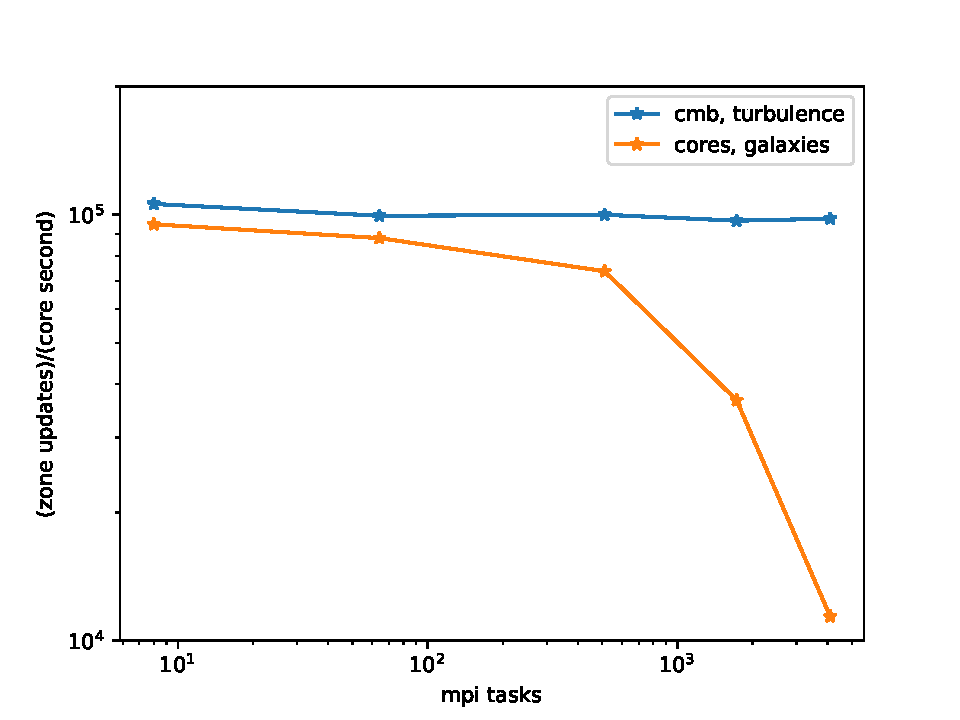
\includegraphics[width=0.99\textwidth]{figs/g49_zoneup.pdf}
\caption[ ]{Zone-pdates per core-second for weak scaling on
    Stampede 2.    
The blue curve only employs
    the MHD solver, in the configuration used for the \nameCMB\ and \nameTurbulence\
    simulations.  The orange curve employs the MHD solver as well as the gravity
    solver and AMR,
 and will be used for the \nameCores\ and \nameGalaxies\ simulations.  The
 gravity and AMR degrade the performance above 512 threads.  This study used 64
 cores per node when possible.}
\label{fig.scaling} \end{center} \end{figure}



\bibliographystyle{apj}
\bibliography{apj-jour,ms.bib}  % looks in ms.bib for bibliography info

\end{document}  


  %dcc 2019 help
%%\input{SUs} %edit beginSU.tex, which has the timing table.  %dcc 2019 help
%%\input{PriorWork}  %dcc 2019 help
%%\input{OtherStuff}  %dcc 2019 help

%\appendix
%\include{ appendix file}


\bibliographystyle{apj}
\bibliography{apj-jour,ms}  % looks in ms.bib for bibliography info
%\bibliography{apj-jour,ms}  % looks in ms.bib for bibliography info

\end{document}  


